Skizzieren Sie alle Mengen in einem Koordinatensystem, und kennzeichnen 
Sie darin die Menge 

\begin{eqnarray}
	\Sigma = A \cap B \cap C \cap D
\end{eqnarray}

	\begin{figure}[h]
		\centering
		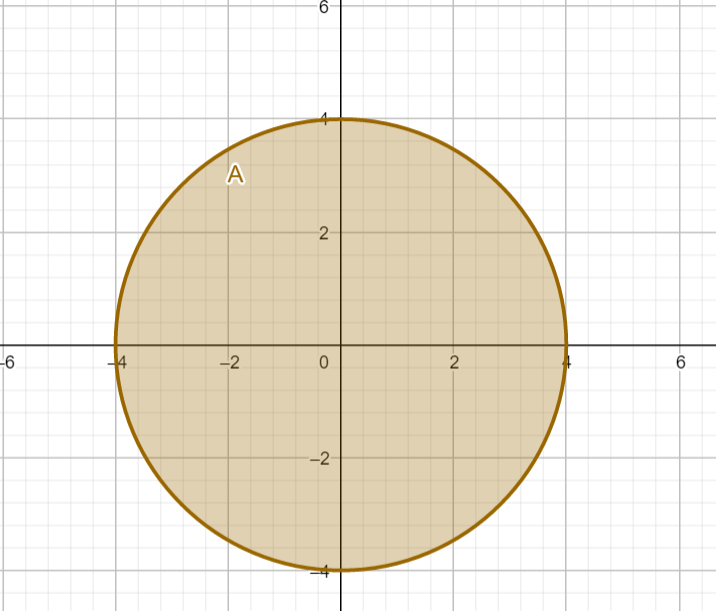
\includegraphics[width=6cm,height=4cm]{MengeA.png}
		\caption{$A = \left\{ \left(x,y \right) \in \mathbb{R} \times \mathbb{R}: x^2 +y^2 \le 16 \right\}$}
		\label{fig:Menge A}
	\end{figure}

	\begin{figure}[h]
	\centering
	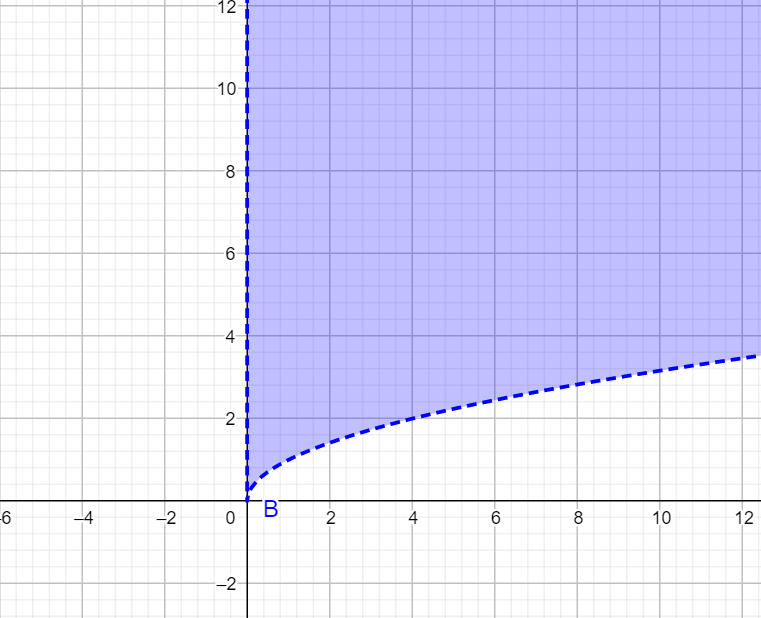
\includegraphics[width=6cm,height=4cm]{MengeB.png}
	\caption{$B=\left\{ \left(x,y \right) \in \mathbb{R_{+}} \times \mathbb{R_{+}}: x > \sqrt{y} \right\}$}
	\label{fig:Menge B}
\end{figure}

\begin{figure}[h]
	\centering
	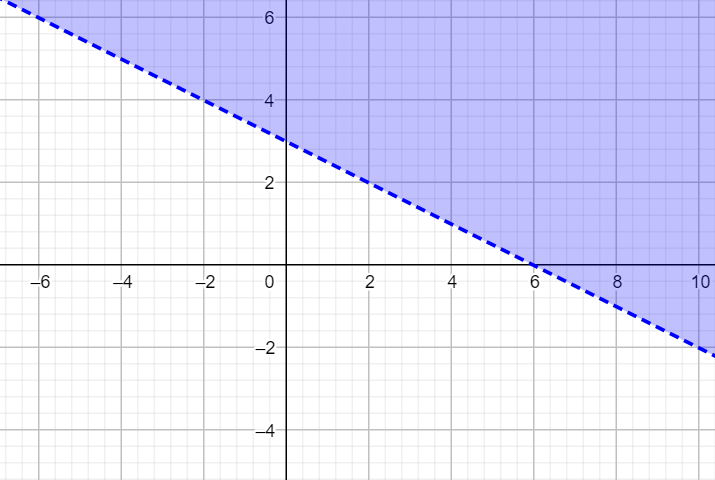
\includegraphics[width=6cm,height=4cm]{MengeC.png}
	\caption{$C = \left\{ \left(x,y \right) \in \mathbb{R} \times \mathbb{R}: y > -\dfrac{1}{2}x+3 \right\}$}
	\label{fig:Menge C}
\end{figure}

\begin{figure}[h]
	\centering
	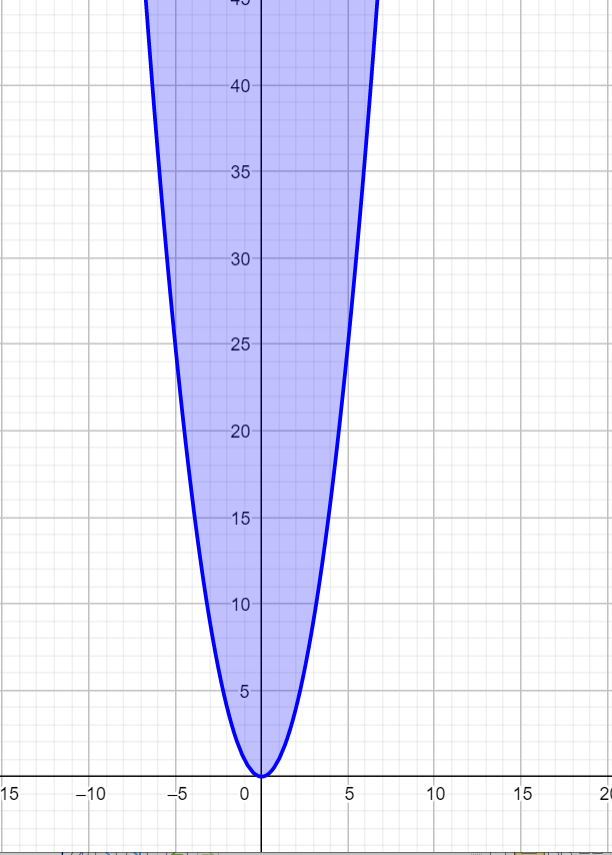
\includegraphics[width=6cm,height=4cm]{MengeD.png}
	\caption{$D = \left\{ \left(x,y \right) \in \mathbb{R} \times \mathbb{R}: y \ge x^2 \right\}$}
	\label{fig:Menge D}
\end{figure}

\begin{figure}[h]
	\centering
	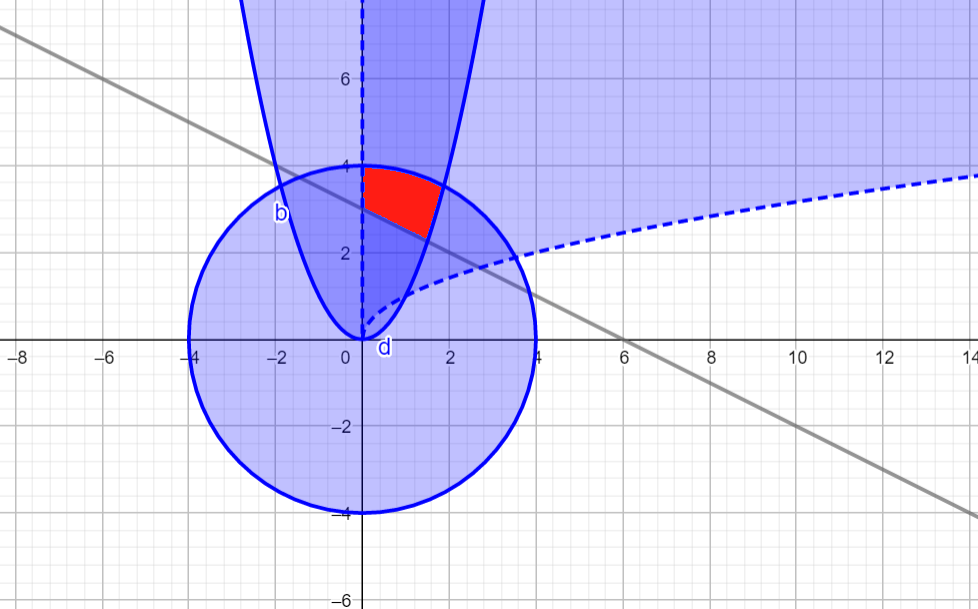
\includegraphics[width=6cm,height=4cm]{MengeE.png}
	\caption{$\Sigma = A \cap B \cap C \cap D$}
	\label{fig:Menge D}
\end{figure}
\clearpage